%% 43장 한 변수 최소화
\chapter{Minimization in One Variable}
\label{ch:scalar-minimization}

\abstract{한 변수 함수의 최솟값을 도함수 없이 찾는 문제는 최적화에서 가장 단순하지만, 그 안에 이 부 전체의 주제가 들어 있다. 확실하지만 느린 방법과 빠르지만 실패할 수 있는 방법이 있고, 좋은 알고리즘은 둘을 섞는다. 이 장에서는 먼저 최솟값을 낀 구간이 무엇인지 정하고, 함수값을 $n$번 계산해 구간을 가장 많이 줄이는 전략이 Fibonacci 탐색이라는 Kiefer의 정리를 증명한다. 그 극한인 황금분할 탐색은 계산 횟수가 많으면 이 최적 전략보다 약 $17\%$ 넓은 구간을 남긴다. 이어서 세 점을 지나는 포물선의 꼭짓점으로 다가가는 포물선 보간의 오차 식을 유도하고, 그 수렴 차수가 $t^3=t+1$의 실근 $1.3247$임을 보인다. 두 방법을 섞은 Brent의 방법을 유사코드로 적고, 매끄러운 함수에서는 황금분할보다 세 배쯤 적은 함수 호출로 같은 정확도에 이르는 것을 확인한다. 끝으로 함수값만으로는 최소점의 위치를 상대 정확도 $\sqrt u$보다 정확히 정할 수 없다는 한계를 수치로 확인하고 구간이 주어진 문제와 배열 원소별 최소화를 다룬다.}

\section{Bracketing a Minimum}
\label{sec:min-bracket}

34장에서 근을 찾을 때는 양 끝의 부호가 다른 구간 하나만 있으면 중간값 정리 덕분에 근이 그 안에 있음이 보장되었다. 최솟값에는 이에 해당하는 정리가 없으므로 함수에 가정을 하나 더한다.

\begin{definition}
함수 $f:[a,b]\to\mathbb R$가 어떤 $x_\ast\in[a,b]$에 대해 $[a,x_\ast]$에서 순감소하고 $[x_\ast,b]$에서 순증가하면 $f$를 $[a,b]$에서 \term{단봉}{unimodal}이라 한다.
\end{definition}

단봉 함수는 연속일 필요가 없고, 최소점 $x_\ast$는 하나뿐이다. 단봉 함수에서는 구간 안의 두 점 $x_1<x_2$의 함수값을 비교하는 것만으로 구간의 일부를 버릴 수 있다. $f(x_1)<f(x_2)$이면 $x_\ast>x_2$일 수 없다. $x_\ast>x_2$라면 $x_1<x_2<x_\ast$에서 $f$가 순감소하므로 $f(x_1)>f(x_2)$가 되어 가정과 어긋난다. 그래서 최소점은 $[a,x_2]$에 있다. 같은 이유로 $f(x_1)>f(x_2)$이면 최소점은 $[x_1,b]$에 있다. 둘이 같으면 최소점은 $[x_1,x_2]$에 있다.

근 찾기와 달리 최소화에는 점이 두 개 필요하다. 근 찾기의 이분법은 가운데 한 점의 부호만 보고 구간을 반으로 줄이지만, 최소화에서는 한 점의 함수값만으로는 아무것도 버릴 수 없다. 대신 한 번 비교한 뒤 남은 구간에는 이미 계산한 점 하나가 안에 들어 있다. $[a,x_2]$가 남으면 $x_1$이, $[x_1,b]$가 남으면 $x_2$가 그 점이다. 그래서 이후로는 새 점 하나만 계산하면 다시 두 점을 비교할 수 있다. 이처럼 구간 $[a,c]$ 안에 한 점 $b$가 있어 $f(b)<f(a)$, $f(b)<f(c)$를 만족하는 세 점을 \term{최솟값을 낀 구간}{bracket of a minimum}이라 한다. 단봉을 가정하지 않아도 $f$가 연속이면 이런 세 점 사이에는 국소 최소점이 있다. $[a,c]$에서 $f$의 최솟값은 $f(b)$ 이하이므로 끝점이 아닌 안쪽에서 얻어지고 그 점이 바로 국소 최소점이다.

\section{Golden-Section Search}
\label{sec:golden-section}

\subsection{The Interval Reduction Ratio}

구간 $[a,b]$의 길이를 $1$로 놓고 안의 두 점을 어디에 둘지 생각해 보자. 어느 쪽이 남을지 모르므로 두 점은 가운데에 대해 대칭으로 두는 것이 자연스럽다. 두 점을 $a+(1-r)$과 $a+r$에 두면($1/2<r<1$) 어느 쪽이 남든 새 구간의 길이는 $r$이다. 남은 구간에는 옛 점 하나가 들어 있는데, 이 점을 다음 단계의 두 점 가운데 하나로 다시 쓰려면 그 점이 새 구간에서도 같은 비율의 자리에 있어야 한다. $[a,a+r]$이 남았다면 옛 점 $a+(1-r)$이 새 구간의 $r$배 자리, 곧 $a+r\cdot r$에 있어야 하므로
\[
r^2=1-r,\qquad r=\frac{\sqrt5-1}2=0.6180339887\ldots
\]
이다. 이 $r$이 황금비 $\varphi=(1+\sqrt5)/2$의 역수이므로 이 방법을 \term{황금분할 탐색}{golden-section search}이라 한다. 첫 두 점을 계산한 뒤에는 함수값을 한 번 계산할 때마다 구간의 길이가 정확히 $r$배가 된다. 이분법이 한 번에 $1/2$배로 줄이는 것과 견주면, 함수값 하나가 주는 정보는 근 찾기보다 적다. 구간의 길이를 $10^{-8}$배로 줄이려면 근 찾기의 이분법은 함수값을 $27$번 계산하면 되지만, 황금분할은 구간을 $\lceil\ln10^{8}/\ln\varphi\rceil=39$번 줄여야 하므로 $40$번 계산한다.

\begin{figure}[t]
\centering
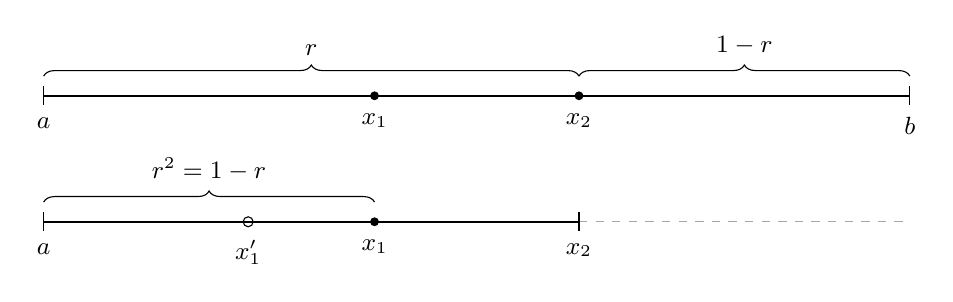
\begin{tikzpicture}[x=11cm, y=1cm, every node/.style={font=\small}]
  \draw[line width=0.6pt] (0,0) -- (1,0);
  \foreach \x/\l in {0/$a$, 1/$b$} {\draw (\x,0.12) -- (\x,-0.12); \node[below] at (\x,-0.15) {\l};}
  \fill (0.381966,0) circle (1.6pt) node[below=3pt] {$x_1$};
  \fill (0.618034,0) circle (1.6pt) node[below=3pt] {$x_2$};
  \draw[decorate, decoration={brace, amplitude=4pt}] (0,0.25) -- node[above=4pt] {$r$} (0.618034,0.25);
  \draw[decorate, decoration={brace, amplitude=4pt}] (0.618034,0.25) -- node[above=4pt] {$1-r$} (1,0.25);
  \begin{scope}[yshift=-1.6cm]
  \draw[line width=0.6pt] (0,0) -- (0.618034,0);
  \draw[black!35, dashed] (0.618034,0) -- (1,0);
  \foreach \x/\l in {0/$a$, 0.618034/$x_2$} {\draw (\x,0.12) -- (\x,-0.12); \node[below] at (\x,-0.15) {\l};}
  \fill (0.381966,0) circle (1.6pt) node[below=3pt] {$x_1$};
  \draw (0.236068,0) circle (1.8pt) node[below=3pt] {$x_1'$};
  \draw[decorate, decoration={brace, amplitude=4pt}] (0,0.25) -- node[above=4pt] {$r^2=1-r$} (0.381966,0.25);
  \end{scope}
\end{tikzpicture}
\caption{황금분할 탐색의 한 단계. 위: 길이 $1$인 구간에서 두 점 $x_1$, $x_2$는 양 끝에서 $1-r$만큼 떨어져 있다. 아래: $f(x_1)<f(x_2)$이어서 $[a,x_2]$가 남으면 옛 점 $x_1$이 새 구간의 오른쪽 점이 되고 새로 계산할 점은 $x_1'$ 하나이다($r^2=1-r$이기 때문이다).}
\label{fig:golden-section}
\end{figure}

\cref{alg:golden}에 scipy와 stardust의 \code{golden} 방법을 정리했다. 시작은 세 점 $a<b<c$의 구간이고, 처음 두 내부 점 가운데 하나로 $b$를 그대로 쓰며 다른 하나는 넓은 쪽에 비율 $1-r$로 놓는다. 그래서 $b$가 황금분할의 자리에 있지 않으면 구간이 정확히 $r$배씩 줄지는 않지만, 걸음마다 구간이 줄어든다는 성질은 그대로이다. 새 점을 $x_2\gets rx_1+(1-r)x_3$처럼 두 점의 볼록 결합으로 계산하는 것은 부동소수점에서도 새 점이 구간 밖으로 나가지 않게 하기 위해서이다. scipy는 $r$을 $0.61803399$로 적어 두는데, 반올림한 이 상수 때문에 비율이 조금 어긋나도 구간을 줄이는 성질은 그대로이다.

\begin{algorithm}[t]
\begin{algorithmic}[1]
\Require 함수 $f$, 최솟값을 낀 구간 $a<b<c$, 허용오차 $\mathrm{tol}$
\Ensure 근사 최소점 $x$
\State $r\gets(\sqrt5-1)/2$, $x_0\gets a$, $x_3\gets c$
\If{$c-b>b-a$}
  \State $x_1\gets b$, $x_2\gets b+(1-r)(c-b)$ \Comment{넓은 쪽에 새 점}
\Else
  \State $x_2\gets b$, $x_1\gets b-(1-r)(b-a)$
\EndIf
\While{$x_3-x_0>\mathrm{tol}\cdot(|x_1|+|x_2|)$}
  \If{$f(x_2)<f(x_1)$}
    \State $x_0\gets x_1$, $x_1\gets x_2$, $x_2\gets rx_1+(1-r)x_3$ \Comment{$[x_1,x_3]$가 남는다}
  \Else
    \State $x_3\gets x_2$, $x_2\gets x_1$, $x_1\gets rx_2+(1-r)x_0$ \Comment{$[x_0,x_2]$가 남는다}
  \EndIf
\EndWhile
\State \Return $x_1$과 $x_2$ 가운데 함수값이 작은 점
\end{algorithmic}
\caption{황금분할 탐색}
\label{alg:golden}
\end{algorithm}

멈춤 판정 $x_3-x_0\le\mathrm{tol}\cdot(|x_1|+|x_2|)$는 구간의 길이를 최소점 크기의 약 $2\,\mathrm{tol}$배와 견주는 상대 판정이다. 기본값은 $\mathrm{tol}=\sqrt{\varepsilon}\approx1.49\times10^{-8}$인데, 이보다 작게 잡아도 소용이 없는 까닭은 \cref{sec:min-accuracy}에서 본다.

\subsection{Optimality of Fibonacci Search}

황금분할은 함수값을 몇 번 계산할지 정해 두지 않을 때 자연스러운 방법이다. 계산 횟수 $n$을 미리 안다면 더 잘할 수 있을까? Kiefer는 1953년에 이 질문에 답했다\cite{kiefer1953}. 답은 Fibonacci 수 $F_1=F_2=1$, $F_{k+2}=F_{k+1}+F_k$로 표현된다.

문제를 정확히 세우자. 단봉 함수 $f$가 $[a,b]$에 주어지고, 점을 하나씩 골라 함수값을 계산하며, 다음 점은 앞의 값들을 보고 고를 수 있다. 점을 $n$개 계산하고 나면, 계산한 점 가운데 함수값이 가장 작은 점 $p$와 그 양옆의 이웃(계산한 점 또는 $a$, $b$) $\ell<p<r$이 정해지고, \cref{sec:min-bracket}의 논증에 따라 최소점은 $[\ell,r]$에 있다. 이 구간을 \term{불확실 구간}{interval of uncertainty}이라 한다. 탐색 전략의 성능은 모든 단봉 함수에 걸친 최악의 경우 불확실 구간의 길이로 잰다. 함수값이 같은 경우는 탐색하는 쪽에 유리하므로, 최악의 경우를 따질 때는 무시해도 된다.

\begin{theorem}[Kiefer]
\label{thm:fibonacci-optimal}
길이 $L$인 구간에서 함수값을 $n\ge1$번 계산하는 어떤 전략도 최악의 경우 불확실 구간의 길이를 $L/F_{n+1}$보다 작게 만들 수 없다. 거꾸로 임의의 $\delta>0$에 대해 최악의 경우에도 그 길이를 $L/F_{n+1}+\delta$ 이하로 만드는 전략이 있다.
\end{theorem}

\begin{proof}
하계부터 보인다. 구간 밖의 점은 더 계산해도 아무 정보를 주지 않으므로, 탐색의 중간 상태는 불확실 구간 $[\ell,r]$과 그 안에서 가장 작은 값을 낸 점 $p$로 요약된다. \term{상대}{adversary}는 지금까지의 값과 모순되지 않는 한 새 점의 값을 마음대로 정한다. $p<s<r$인 새 점 $s$에 대해 상대는 $f(s)<f(p)$(그러면 최소점은 $[p,r]$에 있고 새 상태는 $([p,r],s)$이다)와 $f(s)>f(p)$(새 상태는 $([\ell,s],p)$이다) 가운데 어느 쪽도 고를 수 있다. 구간 밖의 값은 그대로 두고 $[\ell,r]$ 안에서 단조인 조각만 다시 그리면 두 경우 모두 단봉 함수를 만들 수 있기 때문이다. $s<p$인 경우도 대칭이다.

남은 계산 횟수가 $j$인 상태 $([\ell,r],p)$에서 최악의 경우 마지막 불확실 구간의 길이를 $W_j$라 하자. $j$에 대한 귀납법으로 다음을 보인다.
\[
W_j\ge\max\Bigl(\frac{r-\ell}{F_{j+2}},\ \frac{r-p}{F_{j+1}},\ \frac{p-\ell}{F_{j+1}}\Bigr).
\]
$j=0$이면 $W_0=r-\ell$이고 $F_1=F_2=1$이므로 성립한다. $j\ge1$이고 다음 점이 $p<s<r$이라 하자($s$가 구간 밖이거나 $s=p$이면 계산 하나를 버리는 것이므로 더 나빠질 뿐이고, $s<p$는 대칭이다). 상대는 두 결과 가운데 나쁜 쪽을 고를 수 있으므로 $W_j$는 두 새 상태 각각의 하계보다 크다. 새 상태 $([p,r],s)$에는 계산이 $j-1$번 남으므로 귀납 가정의 첫째 항과 둘째 항($s$의 오른쪽 부분)으로 $W_j\ge(r-p)/F_{j+1}$, $W_j\ge(r-s)/F_j$이다. 새 상태 $([\ell,s],p)$에서는 첫째 항과 셋째 항으로 $W_j\ge(s-\ell)/F_{j+1}$, $W_j\ge(p-\ell)/F_j\ge(p-\ell)/F_{j+1}$이다. 이것으로 둘째, 셋째 항이 나온다. 첫째 항은 $(s-\ell)+(r-s)=r-\ell$에서 나온다. 만약 $W_j<(r-\ell)/F_{j+2}$이면
\[
s-\ell<\frac{F_{j+1}}{F_{j+2}}(r-\ell),\qquad r-s<\frac{F_j}{F_{j+2}}(r-\ell)
\]
이고 두 식을 더하면 $r-\ell<(r-\ell)(F_{j+1}+F_j)/F_{j+2}=r-\ell$이 되어 모순이다.

처음에는 계산한 점이 없다. 첫 점 $p$를 계산하면 상태 $([a,b],p)$에 계산이 $n-1$번 남으므로 $W\ge L/F_{n+1}$이다.

상계는 \term{Fibonacci 탐색}{Fibonacci search}이 준다. $n=1$이면 할 일이 없고, $n=2$이면 두 점을 가운데의 양옆에 $\delta$보다 가깝게 두면 된다. $n\ge3$이면 첫 두 점을 $a+LF_{n-1}/F_{n+1}$과 $a+LF_n/F_{n+1}$에 두면 어느 쪽이 남든 길이 $LF_n/F_{n+1}$인 구간에 옛 점 하나가 끝에서 $LF_{n-1}/F_{n+1}$만큼 떨어져 있다. 이 점과 대칭인 자리에 새 점을 두는 일을 되풀이하면 $k$번째 계산 뒤의 구간 길이는 $LF_{n+2-k}/F_{n+1}$이다($F_{n+2-k}=F_{n+1-k}+F_{n-k}$이므로 대칭인 두 점이 구간을 이렇게 나눈다). $n-1$번째 계산 뒤에는 길이가 $2L/F_{n+1}$이고 옛 점이 정확히 가운데 있으므로, 마지막 점을 가운데에서 $\delta$만큼 옮겨 계산하면 남는 구간은 $L/F_{n+1}+\delta$ 이하이다.
\end{proof}

황금분할은 계산 횟수를 몰라도 되는 대신 조금 손해를 본다. 첫 두 점 뒤로 매번 $r=1/\varphi$배씩 줄므로 $n$번 계산 뒤의 길이는 $L\varphi^{-(n-1)}$이다. Binet의 공식 $F_k=(\varphi^k-(-\varphi)^{-k})/\sqrt5$로 최적값과 견주면
\[
\frac{L\varphi^{-(n-1)}}{L/F_{n+1}}=F_{n+1}\varphi^{-(n-1)}\longrightarrow\frac{\varphi^2}{\sqrt5}=1.1708\ldots
\]
이다. $n=10$에서 이미 $1.17085$이다. 계산 횟수를 미리 정해야 하는 번거로움을 없애는 값이 마지막 구간 길이로 $17\%$이고, 계산 횟수로 치면 한 번도 안 된다($\ln1.1708/\ln\varphi\approx0.33$).

\begin{aside}[Kiefer와 탐색 이론]
Jack Kiefer(1924--1981)는 실험 계획법의 최적성 이론으로 더 잘 알려진 통계학자이다. 1953년의 다섯 쪽짜리 논문은 단봉 함수의 최댓값을 찾는 순차 탐색을 최소최대 문제로 세우고 Fibonacci 수로 답을 냈다. 상대가 값을 정한다고 보고 최악의 경우를 따지는 이 논법은 15장에서 비교 정렬의 하한을 얻은 결정 나무 논법과 닮았다. 다만 갈래의 수를 세는 대신 상대가 매번 나쁜 갈래를 골라 남는 구간을 키운다.
\end{aside}

\section{Finding an Initial Bracket}
\label{sec:find-bracket}

황금분할과 다음 절의 방법들은 최솟값을 낀 세 점에서 시작한다. 사용자가 두 점이나 아무 점도 주지 않으면 먼저 그런 세 점을 찾아야 한다. stardust는 scipy의 \code{bracket}을 옮겨 다음과 같이 찾는다. 두 점 $x_a$, $x_b$에서 시작해(주지 않으면 $0$과 $1$) $f(x_a)\ge f(x_b)$가 되도록 이름을 바꾸면 내리막은 $x_a$에서 $x_b$ 쪽이다. 그 방향으로 $x_c=x_b+1.618034(x_b-x_a)$를 계산하고, $f(x_c)<f(x_b)$인 동안 세 점을 앞으로 민다. 미는 걸음은 세 점을 지나는 포물선의 꼭짓점 $w$를 먼저 시도하는데, 너무 멀리 가지 않도록 $x_b+110(x_c-x_b)$에서 자르고, 꼭짓점이 쓸모없으면(포물선이 위로 볼록이거나 꼭짓점이 뒤쪽에 있으면) 황금비만큼 넓힌다. $f(x_b)$가 양 끝보다 작아지면 멈춘다. 이 탐색은 $1{,}000$번 반복의 상한이 있고, 상한에 닿거나 점이 유한하지 않게 되면 구간을 찾지 못했다고 알린다.

포물선 외삽 덕분에 이차 함수에서는 이 탐색이 거의 바로 끝난다. $(x-10)^2$을 $(0,1)$에서 시작하면 $x_c=2.618$ 다음의 꼭짓점이 반올림 오차를 빼면 정확히 $10$이어서 함수값 $5$번으로 $(2.618,\,10.00000000000001,\,21.944)$를 얻는다. $(x-100)^4$은 $7$번, $\cosh(x-50)$은 $15$번이다. 구간을 찾는 비용은 최소점까지의 거리의 로그에 비례해 자라므로, 시작점을 잘 주는 것이 계산을 줄이는 가장 쉬운 방법이다.

\section{Parabolic Interpolation}
\label{sec:parabolic}

\subsection{The Vertex Formula}

황금분할은 함수값의 크기를 보지 않고 대소만 쓴다. 매끄러운 함수라면 최소점 근처에서 이차 함수처럼 생겼으므로, 세 점 $(x_0,f_0)$, $(x_1,f_1)$, $(x_2,f_2)$를 지나는 포물선을 그리고 그 꼭짓점을 다음 점으로 삼는 것이 자연스럽다. 이 방법을 \term{연속 포물선 보간}{successive parabolic interpolation}이라 한다. 29장의 Newton 꼴로 보간 다항식을 쓰면 $p(x)=f_0+f[x_0,x_1](x-x_0)+f[x_0,x_1,x_2](x-x_0)(x-x_1)$이고, $p'(u)=0$에서
\[
u=\frac{x_0+x_1}2-\frac{f[x_0,x_1]}{2f[x_0,x_1,x_2]}
\]
이다. 꼭짓점이 최소점이려면 $f[x_0,x_1,x_2]>0$, 곧 포물선이 아래로 볼록이어야 한다. 실제 구현은 가운데 점 $x_1$을 기준으로 쓴 같은 식
\[
u=x_1-\frac12\,\frac{(x_1-x_0)^2(f_1-f_2)-(x_1-x_2)^2(f_1-f_0)}{(x_1-x_0)(f_1-f_2)-(x_1-x_2)(f_1-f_0)}
\]
을 쓴다. 이렇게 분자와 분모를 따로 계산해 두면 나눗셈을 하기 전에 걸음 $u-x_1$이 받아들일 만한지부터 판정할 수 있다.

\subsection{Error Recurrence and Order of Convergence}

꼭짓점이 최소점에 얼마나 가까운지는 보간 오차의 식에서 나온다. 최소점을 $x_\ast$라 하고 $e_i=x_i-x_\ast$, $e_u=u-x_\ast$라 쓰자.

\begin{theorem}
\label{thm:parabolic-error}
$f$가 $x_\ast$의 근방에서 네 번 연속 미분 가능하고 $f'(x_\ast)=0$, $f''(x_\ast)>0$이라 하자. 서로 다른 세 점 $x_0,x_1,x_2$가 $x_\ast$에 충분히 가까우면 꼭짓점 $u$가 정의되고
\[
e_u=\frac{f'''(x_\ast)}{6f''(x_\ast)}\bigl(e_0e_1+e_0e_2+e_1e_2\bigr)+O\bigl(\max_i|e_i|^3\bigr)
\]
이다.
\end{theorem}

\begin{proof}
보간 오차의 식(29장)에서 $f(x)-p(x)=g(x)\,\omega(x)$이다. 여기서 $g(x)=f[x_0,x_1,x_2,x]$이고 $\omega(x)=(x-x_0)(x-x_1)(x-x_2)$이다. $f\in C^4$이면 $g$는 미분 가능하고 $g'(x)=f[x_0,x_1,x_2,x,x]$이며, 둘 다 평균값 꼴의 표현으로 유계이고 $g(x)\to f'''(x_\ast)/6$이다. 세 점이 $x_\ast$에 가까우면 $f[x_0,x_1,x_2]\to f''(x_\ast)/2>0$이므로 꼭짓점이 정의되고, $f[x_0,x_1]=f'(\xi)=O(\max_i|e_i|)$이므로 꼭짓점 공식에서 $e_u=O(\max_i|e_i|)$이다. 미분해 $x=u$를 넣으면 $p'(u)=0$이므로
\[
f'(u)=g'(u)\,\omega(u)+g(u)\,\omega'(u)
\]
이다. 왼쪽은 평균값 정리로 $f'(u)=f'(u)-f'(x_\ast)=f''(\eta)e_u$이다. 오른쪽에서 $u-x_i=e_u-e_i$이므로
\begin{gather*}
\omega'(u)=(e_u-e_1)(e_u-e_2)+(e_u-e_0)(e_u-e_2)+(e_u-e_0)(e_u-e_1),\\
\omega(u)=(e_u-e_0)(e_u-e_1)(e_u-e_2)
\end{gather*}
이다. 먼저 이 식에서 $|e_u|=O(\max_i|e_i|^2)$를 얻는다. $f''(\eta)$는 $f''(x_\ast)/2$보다 크고, 앞에서 얻은 $e_u=O(\max_i|e_i|)$를 쓰면 오른쪽의 항은 $e_ue_i$ 꼴의 교차항까지 모두 $O(\max_i|e_i|^2)$이기 때문이다. 이것을 다시 넣으면 $\omega'(u)=e_0e_1+e_0e_2+e_1e_2+O(\max|e_i|^3)$, $\omega(u)=O(\max|e_i|^3)$이고, $f''(\eta)=f''(x_\ast)+O(\max|e_i|^2)$, $g(u)=f'''(x_\ast)/6+O(\max|e_i|)$이다. 정리하면 주장의 식이 나온다.
\end{proof}

반복에서는 가장 최근의 세 점 $x_{k-2},x_{k-1},x_k$로 $x_{k+1}$을 만든다. 수렴이 초선형이면 $|e_k|\ll|e_{k-1}|\ll|e_{k-2}|$이므로 세 곱 가운데 $e_{k-1}e_{k-2}$가 지배하고, $K=|f'''(x_\ast)/(6f''(x_\ast))|$라 하면 $K|e_{k+1}|\approx K|e_{k-1}|\cdot K|e_{k-2}|$이다. 로그를 취해 $\epsilon_k=-\log(K|e_k|)$로 두면 선형 점화식
\[
\epsilon_{k+1}=\epsilon_{k-1}+\epsilon_{k-2}
\]
이 된다. 특성방정식은 $t^3=t+1$이고 그 실근 $\rho=1.3247\ldots$가 다른 두 복소근보다 절댓값이 크므로 $\epsilon_k$는 $\rho^k$의 비율로 자란다. 따라서 $|e_{k+1}|\approx C|e_k|^\rho$이고 수렴 차수는 $\rho\approx1.3247$이다. 이 수를 \term{플라스틱 수}{plastic number}라 부른다. 34장의 할선법은 $e_{k+1}\approx Ce_ke_{k-1}$에서 차수 $\varphi\approx1.618$을 얻었는데, 최소화의 점화식에는 가장 최근 오차 $e_k$가 지배항에 들어가지 않아 차수가 낮다. 근 찾기는 $f$의 부호 변화를 바로 보지만 최소화는 $f'$의 정보를 함수값의 차이에서 간접적으로 얻어야 하기 때문이다. 이 반복의 수렴은 Jarratt가 1967년에 분석했다\cite{jarratt1967}.

$e^x-2x$(최소점 $\ln2$)에서 세 점 $0.2$, $1.4$, $1.0$으로 시작해 $400$자리 십진 산술로 반복하면 오차가 $4.6\times10^{-6}$, $2.6\times10^{-8}$, $1.4\times10^{-10}$, $2.0\times10^{-14}$, $6.0\times10^{-19}$, $4.6\times10^{-25}$, $2.0\times10^{-33}$, $4.6\times10^{-44}$으로 줄고, \cref{thm:parabolic-error}의 주요항과의 비는 나열한 걸음에서 모두 $0.99$와 $1.0001$ 사이이다. 이웃한 오차의 로그의 비는 $1.42$, $1.30$, $1.39$, $1.33$, $1.34$, $1.34$, $1.33$으로 $\rho$ 둘레에서 흔들리며 다가간다.

\subsection{Weaknesses of Parabolic Interpolation}

순수한 포물선 보간은 세 가지 이유로 혼자 쓰기 어렵다. 첫째, 세 점이 최소점에서 멀면 포물선이 위로 볼록일 수 있고, 그러면 꼭짓점은 최댓값을 가리킨다. 둘째, 꼭짓점이 이미 있는 점과 거의 겹치면 새 정보가 없고, 셋째 점까지 한 직선 위에 가까워지면 분모가 $0$에 가까워진다. 셋째, 최소점이 퇴화하면 수렴이 선형으로 떨어진다. $f''(x_\ast)=0$인 $(x-1)^4$에서 꼭짓점 공식은 오차에 대해 일차 동차식이 되어 $e_{k+1}\approx\lambda e_k$이고, 그 비 $\lambda$는 $e_k=x_k-1=\lambda^k$를 꼭짓점 공식에 넣어 얻는 방정식 $2\lambda^4+2\lambda^3+\lambda^2-2\lambda-1=0$의 근 $\lambda=0.81509$이다. $100$자리 산술로 반복해도 이웃 오차의 비가 $0.81509$로 수렴하여 황금분할의 $0.618$보다도 느리다. 포물선 보간이 빠른 것은 함수가 최소점 근처에서 이차 함수처럼 생겼을 때뿐이다.

\section{Brent's Method}
\label{sec:brent-min}

Brent는 1973년의 책에서 34장의 근 찾기와 같은 생각으로 황금분할과 포물선 보간을 섞었다\cite{brent1973}. 최솟값을 낀 구간 $[a,b]$를 언제나 유지하고, 포물선 걸음이 믿을 만하면 받아들이며, 아니면 황금분할 걸음을 한다. 이 방법은 다섯 점을 들고 다닌다. $x$는 지금까지 함수값이 가장 작은 점, $w$는 두 번째로 작은 점, $v$는 그 직전의 $w$이다. 포물선은 $x$, $w$, $v$를 지난다.

포물선 걸음을 받아들이려면 꼭짓점 $u=x+p/q$가 $(a,b)$ 안에 있어야 하고 걸음의 크기 $|p/q|$가 직전의 직전 걸음의 크기 $|e|$의 절반보다 작아야 한다. 둘째 조건이 이 방법의 핵심이다. 포물선 걸음이 연달아 받아들여지면 걸음의 크기는 두 걸음마다 반 아래로 줄어든다. 걸음이 그만큼 줄지 않는다면 포물선이 수렴하는 모양을 보이지 않는다는 뜻이므로 황금분할 걸음으로 바꾼다. 직전 걸음이 아니라 그 앞의 걸음과 견주므로, 포물선 걸음이 가끔 한 번쯤 덜 줄어들어도 괜찮다. 앞 절의 점화식에서 보듯 $e_{k+1}$은 $e_k$가 아니라 $e_{k-1}e_{k-2}$로 정해지므로, 포물선 보간의 걸음이 매번 고르게 줄 필요는 없다.

허용오차 $\tau=\mathrm{tol}\cdot|x|+10^{-11}$은 멈춤 판정 $\max(x-a,\,b-x)<2\tau$에도 쓰이고 걸음의 최소 크기를 정하는 데에도 쓰인다. 새 점은 언제나 $x$에서 $\tau$ 이상 떨어지고, 포물선의 꼭짓점이 $a$나 $b$에서 $2\tau$ 안에 떨어지면 대신 $x$에서 가운데 쪽으로 $\tau$만 간다. 함수값을 너무 가까운 두 점에서 비교하면 반올림 오차가 차이를 삼켜 버리기 때문이다. 절대 항 $10^{-11}$은 최소점이 $0$ 근처일 때 $\tau$가 $0$이 되는 것을 막는다.

\begin{algorithm}[t]
\begin{algorithmic}[1]
\Require 함수 $f$, 최솟값을 낀 세 점 $a<x<b$, 허용오차 $\mathrm{tol}$
\Ensure 근사 최소점 $x$
\State $w\gets v\gets x$, $e\gets0$, $d\gets0$, $c\gets(3-\sqrt5)/2$
\Loop
  \State $m\gets(a+b)/2$, $\tau\gets\mathrm{tol}\cdot|x|+10^{-11}$
  \If{$\max(x-a,b-x)<2\tau$} \Return $x$ \EndIf
  \State 황금분할을 쓰기로 둔다
  \If{$|e|>\tau$} \Comment{$x$, $w$, $v$를 지나는 포물선}
    \State 꼭짓점으로 가는 걸음 $p/q$를 계산한다
    \If{$a<x+p/q<b$이고 $|p/q|<|e|/2$}
      \State $e\gets d$, $d\gets p/q$, 황금분할을 쓰지 않기로 바꾼다
      \If{$x+d$가 $a$나 $b$에서 $2\tau$ 안이면} $d\gets\tau\cdot\operatorname{sign}(m-x)$ \EndIf
    \EndIf
  \EndIf
  \If{황금분할을 쓰기로 했으면}
    \State $e\gets(a-x$ 또는 $b-x$ 가운데 $x$에서 먼 쪽$)$, $d\gets c\cdot e$
  \EndIf
  \State $u\gets x+\operatorname{sign}(d)\max(|d|,\tau)$ \Comment{적어도 $\tau$만큼 움직인다}
  \If{$f(u)\le f(x)$}
    \State $u$의 반대쪽 끝을 $x$로 옮기고 $(v,w,x)\gets(w,x,u)$
  \Else
    \State $u$ 쪽 끝을 $u$로 옮기고, $f(u)$가 $f(w)$ 이하이면 $(v,w)\gets(w,u)$, 아니고 $f(v)$ 이하이면 $v\gets u$
  \EndIf
\EndLoop
\end{algorithmic}
\caption{Brent의 한 변수 최소화}
\label{alg:brent-min}
\end{algorithm}

\cref{alg:brent-min}이 그 전체이다. 황금분할 걸음은 $x$에서 구간의 넓은 쪽으로 그 길이의 $c=0.381966$배만큼 간다. 새 점이 $x$와 먼 끝 사이를 $c:(1-c)$로 나누므로 이것은 \cref{sec:golden-section}의 황금분할과 같은 비율이다. 함수값 비교는 같을 때 새 점 $u$를 택한다($f(u)\le f(x)$). $w=x$나 $v=x$ 같은 겹침을 따지는 조건은 처음 몇 걸음에 세 점이 아직 다 다르지 않을 때를 다룬다.

\begin{figure}[t]
\centering
\begin{tikzpicture}
\begin{semilogyaxis}[sdplot, xlabel={함수값 계산 횟수}, ylabel={가장 좋은 점의 오차}, xmin=0, xmax=46, ymin=1e-13, ymax=2, legend pos=north east, height=0.5\textwidth]
\fill[black!8] (axis cs:0,1e-13) rectangle (axis cs:46,6.8e-9);
\addplot+[no marks, const plot] coordinates {(1,6.93e-01) (2,3.07e-01) (3,3.07e-01) (4,7.51e-02) (5,7.51e-02) (6,7.51e-02) (7,7.08e-02) (8,7.08e-02) (9,1.51e-02) (10,1.51e-02) (11,1.51e-02) (12,1.90e-03) (13,1.90e-03) (14,1.90e-03) (15,1.20e-03) (16,1.20e-03) (17,1.82e-05) (18,1.82e-05) (19,1.82e-05) (20,1.82e-05) (21,1.82e-05) (22,1.82e-05) (23,1.82e-05) (24,1.82e-05) (25,1.82e-05) (26,2.64e-06) (27,2.64e-06) (28,2.64e-06) (29,1.05e-06) (30,1.05e-06) (31,3.61e-07) (32,3.61e-07) (33,1.77e-07) (34,1.77e-07) (35,2.85e-08) (36,2.85e-08) (37,2.85e-08) (38,2.85e-08) (39,1.45e-09) (40,1.45e-09) (41,1.45e-09) (42,1.45e-09) (43,1.45e-09) (44,1.45e-09) (45,1.45e-09)};
\addlegendentry{황금분할}
\addplot+[no marks, const plot] coordinates {(1,6.93e-01) (2,6.93e-01) (3,3.07e-01) (4,9.77e-02) (5,3.66e-02) (6,3.60e-03) (7,5.63e-04) (8,2.50e-05) (9,3.55e-07) (10,2.31e-09) (11,2.31e-09) (12,1.15e-09) (13,1.15e-09)};
\addlegendentry{포물선 보간}
\addplot+[no marks, const plot] coordinates {(1,6.93e-01) (2,3.07e-01) (3,3.07e-01) (4,7.51e-02) (5,7.51e-02) (6,1.62e-02) (7,5.12e-03) (8,1.26e-04) (9,1.41e-05) (10,9.49e-08) (11,2.88e-10) (12,2.88e-10) (13,2.88e-10) (14,1.91e-12) (15,1.91e-12) (16,1.91e-12) (17,1.91e-12) (18,1.91e-12) (19,1.91e-12)};
\addlegendentry{Brent}
\end{semilogyaxis}
\end{tikzpicture}
\caption{$e^x-2x$의 최소점 $\ln2$를 찾을 때 계산 횟수에 따른 가장 좋은 점의 오차. 황금분할과 Brent는 세 점 $(0,1,2)$에서, 포물선 보간은 $0$, $2$, $1$에서 시작했고, 앞의 세 번은 시작점의 계산이다. 황금분할과 Brent는 허용오차를 $10^{-15}$로 낮추어 끝까지 돌렸다. 회색 띠는 계산한 함수값이 최솟값과 구별되지 않는 범위(\cref{sec:min-accuracy})로, 그 안의 오차의 크기는 우연이다.}
\label{fig:min-convergence}
\end{figure}

\cref{fig:min-convergence}는 세 방법을 견준다. 황금분할은 구간이 일정하게 줄어도 가장 좋은 점이 가끔씩만 바뀌므로 오차가 계단 모양으로 줄어든다. 포물선 보간과 Brent는 초선형으로 떨어지다가 회색 띠에 들어가면 더 나아지지 않는다. Brent의 처음 두 걸음은 황금분할인데, 첫 걸음에서는 $e=0$이어서 포물선을 시도하지 않고 둘째 걸음에서는 $x$, $w$, $v$ 가운데 둘이 아직 같아 포물선이 정해지지 않는다. 이후로는 포물선 걸음이 받아들여져 순수한 포물선 보간과 거의 같은 속도로 줄어든다.

\cref{tab:min-counts}에는 네 함수에서 기본 허용오차로 멈출 때까지의 계산 횟수를 재어 실었다. 계산 횟수에는 시작한 세 점이 들어 있고, 오차는 돌려준 점과 참 최소점의 거리이다. 매끄러운 두 함수에서 Brent는 황금분할보다 세 배쯤 적게 계산한다. 꺾인 점이 최소점인 $|x-0.3|$에서는 포물선이 맞지 않아 황금분할 걸음이 섞이지만 그래도 덜 계산한다. 퇴화한 최소점 $(x-1)^4+1$에서는 두 방법 모두 오차가 $10^{-4}$에 머무는데, 그 까닭은 다음 절에서 본다. 이 값들은 scipy 1.18.1의 같은 방법으로도 계산 횟수와 결과가 모두 같았다.

\begin{table}[t]
\begin{sdtable}{colspec={lcccc}, row{1}={font=\small\bfseries}}
\toprule
함수(시작한 세 점) & 황금분할 횟수 & 황금분할 오차 & Brent 횟수 & Brent 오차 \\
\midrule
$e^x-2x$ $(0,1,2)$ & $43$ & $1.4\times10^{-9}$ & $15$ & $1.1\times10^{-8}$ \\
$-xe^{-x}$ $(0,2,5)$ & $45$ & $2.0\times10^{-9}$ & $15$ & $1.4\times10^{-9}$ \\
$|x-0.3|$ $(0,0.5,1)$ & $44$ & $6.4\times10^{-10}$ & $30$ & $1.5\times10^{-9}$ \\
$(x-1)^4+1$ $(0,1.5,3)$ & $43$ & $1.0\times10^{-4}$ & $38$ & $1.0\times10^{-4}$ \\
\bottomrule
\end{sdtable}
\caption{기본 허용오차(황금분할 $\sqrt\varepsilon$, Brent $1.48\times10^{-8}$)로 멈출 때까지 함수값을 계산한 횟수와 돌려준 점의 오차.}
\label{tab:min-counts}
\end{table}

Brent의 오차가 $e^x-2x$에서 황금분할보다 큰 것은 이상하지 않다. 두 방법 모두 구간의 길이가 허용오차에 닿을 때 멈추고, 그때 돌려준 점이 구간 안의 어디에 있는지는 마지막 걸음들의 우연에 달려 있다. 보장되는 것은 오차가 대략 $\mathrm{tol}\cdot|x_\ast|$ 정도라는 것뿐이다.

\section{Attainable Accuracy}
\label{sec:min-accuracy}

42장에서 함수값만 써서는 최소점의 위치를 대략 $\sqrt u$의 상대 정확도보다 정확히 정할 수 없다고 했다. 한 변수에서 이것을 수치로 확인해 보자. 최소점 근처에서 $f(x_\ast+h)-f(x_\ast)\approx f''(x_\ast)h^2/2$이고, 계산한 $f$의 값은 상대오차 $u$ 정도로 흔들리므로 $f''h^2/2$가 $u|f(x_\ast)|$보다 작은 $h$에서는 두 값을 구별할 수 없다. 구별할 수 없는 범위의 반지름은
\[
|h|\approx\sqrt{\frac{2u|f(x_\ast)|}{f''(x_\ast)}}
\]
이다. $e^x-2x$에서는 $f(x_\ast)=2-2\ln2\approx0.614$, $f''(x_\ast)=2$이므로 $8.3\times10^{-9}$이다. 실제로 binary64의 $\ln2$ 둘레에서 $10^{-12}$ 간격으로 계산해 보면, 가장 작은 계산값 $0.6137056388801092$가 $x_\ast+10^{-12}$부터 $x_\ast+6.8\times10^{-9}$까지 여기저기서 나오고, 그 값에서 $2$ ULP 이내인 점은 $|h|\le1.6\times10^{-8}$까지 퍼져 있다. 이 범위 안에서는 함수값 비교가 반올림의 우연에 따라 갈리므로 어떤 비교 기반 방법도 최소점을 더 좁힐 수 없다. \cref{fig:min-convergence}의 회색 띠가 이 범위이고, Brent가 $1.9\times10^{-12}$에 이른 것은 운이 좋았을 뿐이다. Brent의 기본 허용오차 $1.48\times10^{-8}$은 $\sqrt{2.2\times10^{-16}}$, 곧 $\sqrt\varepsilon$이다. 이보다 작게 잡으면 계산만 늘고 정확도는 나아지지 않는다.

최소점이 퇴화하면 한계는 더 나빠진다. $f(x_\ast+h)-f(x_\ast)\approx ch^4$이면 구별할 수 없는 범위가 $(u|f(x_\ast)|/c)^{1/4}$이다. $(x-1)^4+1$을 binary64로 계산하면 $|h|\le1.026\times10^{-4}$인 모든 $x=1+h$에서 값이 정확히 $1$이며 이 범위는 $u^{1/4}=(2^{-53})^{1/4}\approx1.026\times10^{-4}$와 맞는다. \cref{tab:min-counts}의 마지막 줄에서 두 방법의 오차가 $10^{-4}$에 머문 것도 이 때문이다.

도함수를 계산할 수 있다면 이 한계를 피할 수 있다. 최소점은 $f'(x)=0$의 근이고, $f'(x_\ast+h)\approx f''(x_\ast)h$는 $h$에 비례하므로 34장의 근 찾기는 $u$에 가까운 정확도를 낸다. $e^x-2=0$을 구간 $[0,2]$에서 Brent의 근 찾기로 풀면 오차가 $1.1\times10^{-16}$, 곧 상대오차 $1.6\times10^{-16}$이다. 다만 $f'=0$은 최대점과 변곡점에서도 성립하므로, 구간 안에서 $f'$이 음에서 양으로 바뀌는지 확인해야 한다. 함숫값의 크기가 아니라 위치가 필요할 때는 이 차이가 크다. 최대우도 추정에서 추정량 자체가 궁금하면 점수 함수의 근을 찾는 것이 우도를 직접 최적화하는 것보다 대략 여덟 자리를 더 준다.

\section{Bounded Problems}
\label{sec:bounded}

최소점을 정해진 구간 $[x_1,x_2]$에서 찾아야 하는 경우도 많다. 모수의 범위가 제한된 최대우도 추정이 그렇다. scipy의 \code{fminbound}와 그것을 옮긴 stardust의 \code{bounded} 방법은 Brent의 책에 실린 원래 알고리즘이고(Forsythe, Malcolm, Moler가 이것을 Fortran으로 옮긴 것이 \code{fmin}이다), \cref{alg:brent-min}과는 시작만 다르다\cite{brent1973,forsythe1977}. 최솟값을 낀 세 점에서 시작하지 않고, 원래 알고리즘대로 첫 점을 황금분할의 자리 $x_1+0.381966(x_2-x_1)$에 두어 그 한 점에서 시작한다. 처음에는 $e=0$이어서 첫 두 걸음은 황금분할이고, 그 뒤로는 \cref{alg:brent-min}과 같다.

다만 다른 점이 둘 있다. 첫째, 끝점에서는 함수를 계산하지 않는다. 새 점은 끝점과 겹치지 않고 끝에서 대략 $\tau$ 이상 떨어지므로 끝점에서 정의되지 않는 함수(예컨대 $\log x$를 담은 우도를 $[0,1]$에서)도 다룰 수 있다. 최소점이 끝점이면 그 끝에서 허용오차만큼 떨어진 점에 수렴한다. $f(x)=x$를 $[0,1]$에서 최소화하면 함수값 $25$번 뒤에 $x=6.0\times10^{-6}$을 돌려준다. 둘째, 허용오차가 $\tau=\sqrt{2.2\times10^{-16}}\,|x|+\mathrm{xatol}/3$으로 절대 항을 사용자가 정하고, 그 기본값이 $\mathrm{xatol}=10^{-5}$이다. 이 값은 상대 정확도로 치면 꽤 거칠다. $e^x-2x$를 $[0,2]$에서 기본값으로 풀면 함수값 $9$번으로 오차 $7.3\times10^{-8}$에 멈추고, $\mathrm{xatol}=10^{-12}$로 낮추면 $13$번으로 $1.0\times10^{-8}$에 이른다. 그 아래로는 앞 절의 한계 때문에 더 나아지지 않는다.

\section{Elementwise Minimization over Arrays}
\label{sec:batch-min}

모수가 다른 같은 꼴의 문제를 많이 풀어야 할 때가 있다. 예컨대 관측마다 다른 한 변수 우도를 최대화하는 경우이다. 문제마다 Python 함수를 따로 부르면 호출 비용이 계산을 압도하므로, 반복마다 아직 끝나지 않은 모든 원소의 점을 배열 하나에 모아 사용자 함수를 한 번 부르는 것이 낫다. 이렇게 하려면 원소마다 걸음이 달라도 한 반복에 함수값 하나씩을 쓰는 방법이 필요하다. scipy의 \code{elementwise.find\_minimum}과 stardust의 \code{find\_minimum}은 Chandrupatla가 1998년에 낸 방법을 쓴다\cite{chandrupatla1998}. 34장의 배열 근 찾기가 쓰는 Chandrupatla의 1997년 방법과 짝이다.

Chandrupatla의 방법은 Brent와 같은 생각을 더 간결한 규칙에 담는다. 세 점 $x_1,x_2,x_3$는 가운데 $x_2$에서 함수값이 가장 작고, 넓은 쪽이 $x_3$가 되도록 이름을 바꾸어 둔다. 포물선의 꼭짓점 $q$를 계산해 직전 반복의 꼭짓점 $q_{\mathrm{prev}}$와 $|q-q_{\mathrm{prev}}|<|x_2-x_1|/2$이면 받아들이고, 아니면 넓은 쪽으로 황금분할 걸음 $x_2+0.381966(x_3-x_2)$를 한다. 꼭짓점이 연이어 같은 곳을 가리키면 포물선이 자리를 잡았다고 보는 셈이다. 꼭짓점이 $x_2$에서 허용오차 안이면 그만큼 밀어낸다. 반복은 넓은 쪽의 길이가 $|x_3-x_2|\le2(\mathrm{xrtol}\cdot|x_2|+\mathrm{xatol})$이 되거나, 이계 차분 $f_1-2f_2+f_3$이 $2(\mathrm{frtol}\cdot|f_2|+\mathrm{fatol})$ 이하가 되면 멈춘다. 뒤의 판정은 세 함수값이 더는 구별되지 않는 앞 절의 평평한 영역에 들어왔음을 알린다. 기본값은 $\mathrm{xrtol}=\sqrt\varepsilon$이고 나머지는 가장 작은 정규 수이다.

$e^x-2x$를 $(0,1,2)$에서 시작하면 $13$번 반복, 함수값 $16$번으로 오차 $8.7\times10^{-10}$에 멈추고, $|x-0.3|$은 $27$번 반복, $30$번으로 오차 $1.5\times10^{-9}$이다. 원소 하나만 보면 Brent와 비슷한 효율이다.

\begin{instardust}[\code{docs/design/optimize.md} §3.2, §3.3]
\code{sd.optimize.minimize\_scalar}는 \code{method}로 \code{'brent'}, \code{'golden'}, \code{'bounded'}를 고르고, \code{bounds}를 주면 기본이 \code{'bounded'}, 아니면 \code{'brent'}이다. 기본 허용오차와 반복 상한은 scipy와 같다(brent $1.48\times10^{-8}$과 $500$번, golden $\sqrt\varepsilon$과 $5{,}000$번, bounded는 $\mathrm{xatol}=10^{-5}$와 함수값 $500$번). 세 방법은 C++ 커널(\code{csrc/optimize/scalar.cpp})이 scipy의 Python 구현을 같은 순서의 연산으로 옮긴 것이어서, 설계 문서는 기록한 $399$번의 실행에서 사용자 함수를 부른 점이 scipy 1.18.1과 비트까지 같다고 적는다. scipy의 이 세 방법은 Python이라 FMA가 없고, stardust는 컴파일러의 축약을 끄므로 같은 결과가 나온다. 결과의 \code{status}는 $0$ 수렴, $1$ 반복 상한, $2$ NaN에 더해, scipy가 예외로 알리던 구간 찾기의 실패를 $3$(구간을 못 찾음)과 $4$(구간 찾기의 반복 상한)로 돌려주고, 그때는 그때까지의 세 점 가운데 가장 낮은 점을 \code{converged=False}로 준다. 배열 함수 \code{find\_minimum}과 \code{bracket\_minimum}은 반복마다 남은 원소를 새 배열에 모아 함수를 한 번 부르고, 남은 원소가 $2^{15}$개 이상이면 원소별 갱신을 스레드에 나눈다.
\end{instardust}

\section{Concluding Remarks}

한 변수 최소화는 이 부의 축소판이다. 황금분할은 단봉이라는 가정 하나로 수렴을 보장하고, Kiefer의 정리는 그 보장이 거의 최선임을 말한다. 포물선 보간은 함수가 이차 함수를 닮았다는 데 기대어 초선형으로 수렴하지만, 그 가정이 깨지면 황금분할보다도 느려진다. Brent의 방법은 걸음의 크기를 지켜보며 두 방법 사이를 오가서 황금분할의 안전성과 포물선 보간의 속도를 함께 얻는다. 다음 장들의 다변수 방법도 같은 짜임이다. 빠른 모형 걸음(Newton, 준Newton)을 안전 장치(선 탐색, 신뢰 영역)가 감싼다. 함수값만 쓰는 한 어느 방법이든 위치의 정확도가 $\sqrt u$에 막힌다는 사실도 그대로 이어진다.

도함수 없는 한 변수 최소화의 고전은 Brent의 책\cite{brent1973}으로, \code{fmin}의 원본인 Algol 절차 \code{localmin}과 수렴 논증이 함께 실려 있다. 탐색 이론의 최소최대 관점은 Kiefer의 논문\cite{kiefer1953}에서 시작되었다.

\chapterreferences
